% Paper 2015
\documentclass[12pt,journal]{IEEEtran}

% *** MISC UTILITY PACKAGES ***
%
\usepackage{ifpdf}
% Heiko Oberdiek's ifpdf.sty is very useful if you need conditional
% compilation based on whether the output is pdf or dvi.
% usage:
% \ifpdf
   % pdf code
 %\else
   % dvi code
% \fi

% *** CITATION PACKAGES ***
%
\usepackage{cite}

% *** GRAPHICS RELATED PACKAGES ***
%
\ifCLASSINFOpdf
   \usepackage[pdftex]{graphicx}
  % declare the path(s) where your graphic files are
   \graphicspath{{../pdf/}{../jpeg/}}
  % and their extensions so you won't have to specify these with
  % every instance of \includegraphics
   \DeclareGraphicsExtensions{.pdf,.jpeg,.png}
\else
  % or other class option (dvipsone, dvipdf, if not using dvips). graphicx
  % will default to the driver specified in the system graphics.cfg if no
  % driver is specified.
   \usepackage[dvips]{graphicx}
  % declare the path(s) where your graphic files are
  \graphicspath{{../eps/}}
  % and their extensions so you won't have to specify these with
  % every instance of \includegraphics
   \DeclareGraphicsExtensions{.eps}
\fi

% *** MATH PACKAGES ***
%
\usepackage[cmex10]{amsmath}

% *** SPECIALIZED LIST PACKAGES ***
%
\usepackage{algorithmic}

% *** ALIGNMENT PACKAGES ***
%
\usepackage{array}


% *** SUBFIGURE PACKAGES ***
\ifCLASSOPTIONcompsoc
  \usepackage[caption=false,font=normalsize,labelfont=sf,textfont=sf]{subfig}
\else
  \usepackage[caption=false,font=footnotesize]{subfig}
\fi

% *** FLOAT PACKAGES ***
%
\usepackage{fixltx2e}

\usepackage{stfloats}

\ifCLASSOPTIONcaptionsoff
  \usepackage[nomarkers]{endfloat}
 \let\MYoriglatexcaption\caption
\renewcommand{\caption}[2][\relax]{\MYoriglatexcaption[#2]{#2}}
\fi

% *** PDF, URL AND HYPERLINK PACKAGES ***
%
\usepackage{url}


\usepackage{siunitx}
\DeclareSIUnit\photon{\ensuremath{\gamma}}
\DeclareSIUnit\proton{p}
\DeclareSIUnit\neutron{n}
\usepackage{booktabs}
\usepackage{graphicx}
\usepackage{epstopdf}
\usepackage{subfig}

\usepackage{todo}
% correct bad hyphenation here
\hyphenation{op-tical net-works semi-conduc-tor}


\begin{document}
%----------------------------------------------------------------------------------------
%	TITLE SECTION
%----------------------------------------------------------------------------------------
\title{Monte Carlo calculation to characterize neutron and gamma fields for ANITA neutron facility at TSL}

\author{Q. Hong,
S. P. Platt,~\IEEEmembership{Member,~IEEE}
Alexander V. Prokofiev,~\IEEEmembership{Member,~IEEE}
\thanks{further information}\\[2mm] 	% Your name
%\normalsize University of Central Lancashire \\ 							% Your institution
%\normalsize \href{qhong@uclan.ac.uk} 								% Your email address
\vspace{-5mm}
}


%----------------------------------------------------------------------------------------

\maketitle % Insert title

%----------------------------------------------------------------------------------------
%	ABSTRACT
%----------------------------------------------------------------------------------------

\begin{abstract}
Monte Carlo simulation of spallation neutron source of ANITA at TSL was used to analyze radiation fields at the Close User Position (CUP) and Standard User Position(SUP) for single-event effect testing. ...
\end{abstract}

%----------------------------------------------------------------------------------------
%	KEYWORDS
%----------------------------------------------------------------------------------------
\begin{IEEEkeywords}
ANITA,Geant4, neutron,gamma, TSL.
\end{IEEEkeywords}

%----------------------------------------------------------------------------------------
%	ARTICLE CONTENTS
%----------------------------------------------------------------------------------------

\IEEEpeerreviewmaketitle

\section{Introduction}

\IEEEPARstart{M}{onte} Carlo simulations of naked spallation neutron sources at Los Alamos Neutron Science Center (LANSCE) Weapons Neutron Research (WNR) Target 4\cite{Wender87} and the ANITA beam at the University of Uppsala The Svedberg Laboratory (TSL) have been completed using Geant4 and proved that Binary intranuclear cascade (INC) model gave a good representation of neutron spectra than Bertini INC model did\cite{Platt13}. Simulation result of neutron spectra using Geant4 with Binary INC model is below measurement data from ANITA neutron facility. It is likely to be influenced by our omission of collimator, shielding, and bending magnet component. This work is to verify this hypothesis is correct. In addition, we are intested in the gamma field at CUP and SUP in spallation neutron source at the ANITA neutron facility at TSL for SEE testing.
%------------------------------------------------

\section{Modelling}

A detailed model of the ANITA geometry was implemented in Geant4.
This is illustrated in overview in Fig.~\ref{fig:ANITAoverview}
Description of the geometry is given in \cite{Prokofiev2009,Prokofiev14}; a summary only is given here.
The spallation target is a tungsten cylinder of diameter \SI{0}{\cm} and length \SI{0}{\cm}.
The target is cooled by water and surrounded by a stainless-steel cooling jacket.
The target assembly with its cooling jacket appears as a small blue rectangle in Fig.~\ref{fig:ANITAoverview}.
Lead shielding blocks in the target region are also modelled, and shown in red Fig.~\ref{fig:ANITAoverview}.
A large electromagnet surrounding the target is modelled and shown in Fig.~\ref{fig:ANITAoverview} in grey (iron) and yellow (copper).
An iron collimator with variable apertures is modelled  and shown downstream of the target (grey).

\begin{figure}[!t]
	\centering
	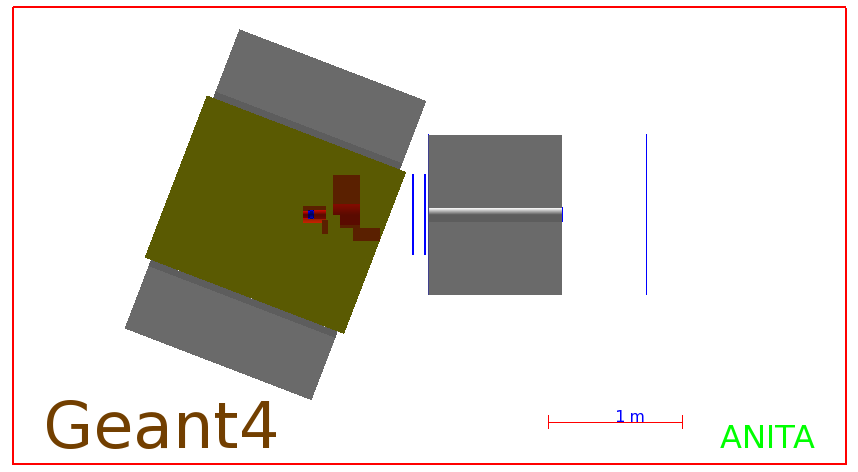
\includegraphics[width=3in]{overview.png}
	\caption{Simulated ANITA facility overview seen from above (yellow: bending magnet; red: shielding components; blue: target cooling jacket (enclosing the target); grey: collimator; blue: detector system)}
	\label{fig:ANITAoverview}
\end{figure}

Simulations were conducted using Geant4 version~TBD.
The TBD intranuclear cascade model was selected in accordance with the results of earlier work~\cite{Platt13}, in which it performed well in simulations of neutron spallation in the region from \SIrange{0}{0}{\MeV}.
In the simulation protons were incident axially at an energy of \SI{180}{\MeV}.
Resulting gamma and neutron fields were evaluated at several locations.
In this paper results are presented for three of these: The Standard User Position (SUP), \SI{2.5}{\m} downstream of the target centre (check centre)~\cite{Prokofiev2009}, the Close User Position (CUP), \SI{0}{\m} downstream of the target, and the CUP-TOF, \SI{0}{m} downstream of the target.
The SUP, CUP and CUP-TOF positions are visible in blue in Fig.~\ref{fig:ANITAoverview}.
The SUP and CUP positions are of interest as they are positions used for SEE tests; the CUP-TOF position is the location of thin-film breakdown counter (TFBC) detectors used for beam monitoring and characterisation using time-of-flight (TOF) techniques.
Model validation will be demonstrated against CUP-TOF data (section~\ref{tbd}).



\begin{table}[!tbp]
\caption{Neutron yield under the umbra region at the standard user position}	%title of the table
	\label{table:NYieldRadiusEffectAtSUP}
	\centering
	\begin{tabular}{l c c c}
		\toprule
          {collimator}   		&{$< \SI{1}{\MeV}$}	&{$\geq 1 \& <\SI{10}{\MeV}$}	&{$\geq \SI{10}{\MeV}$}\\
          \cmidrule(r){2-4}
          {\si{\centi\metre}}	&						&{\SI{1e-6}{\neutron\per\cm\squared\per\proton}}	&\\
          \midrule
		3 		& 0.833 	& 0.975	& 0.525\\
		10.2 	& 1.394 	& 1.248	& 0.525\\
		30 		& 1.962 	& 1.555	& 0.650\\
           \bottomrule
	\end{tabular}
\end{table}

%------------------------------------------------
\section{Results}

In previous work Platt et al.~\cite{Platt13} reported simulations of a naked ANITA target, demonstrating good qualitative agreement with independent calculations and measurements of the fast neutron field at ANITA SUP~\cite{Prokofiev2009}.
Part of the motivation for this work was to investigate whether improvements in the fidelity of the Geant4 model would lead to increased quantitative agreement.
Fig.~\ref{fig:SUPCollimator}

\begin{figure}
    \todo{}
    \caption{Neutron field at the Standard User Position downstream of the \SI{10.2}{\cm} collimator}
    \label{fig:SUPCollimator}
\end{figure}

\begin{figure}
    \todo{}
    \caption{Neutron profile at the Standard User Position downstream of the \SI{10.2}{\cm} collimator}
    \label{fig:SUPProfile}
\end{figure}

Fig.~\ref{fig:FirstComparison}\ldots

\begin{figure}
	\todo{Here we need figures showing the integral spectra on log-log plots and equilethargic spectra normalised to unit area above \SI{10}{\MeV}}
	\caption{Neuton spectrum at the SUP, showing comparison between the standard facility parameterisation~\cite{Prokofiev2009} and results from a naked Geant4 model~\cite{Platt13} and this work.}
	\label{fig:FirstComparison}
\end{figure}

\subsection{Subsection One}
\begin{figure*}[!t]
	\centering
	\subfloat[Geant4 modelling]{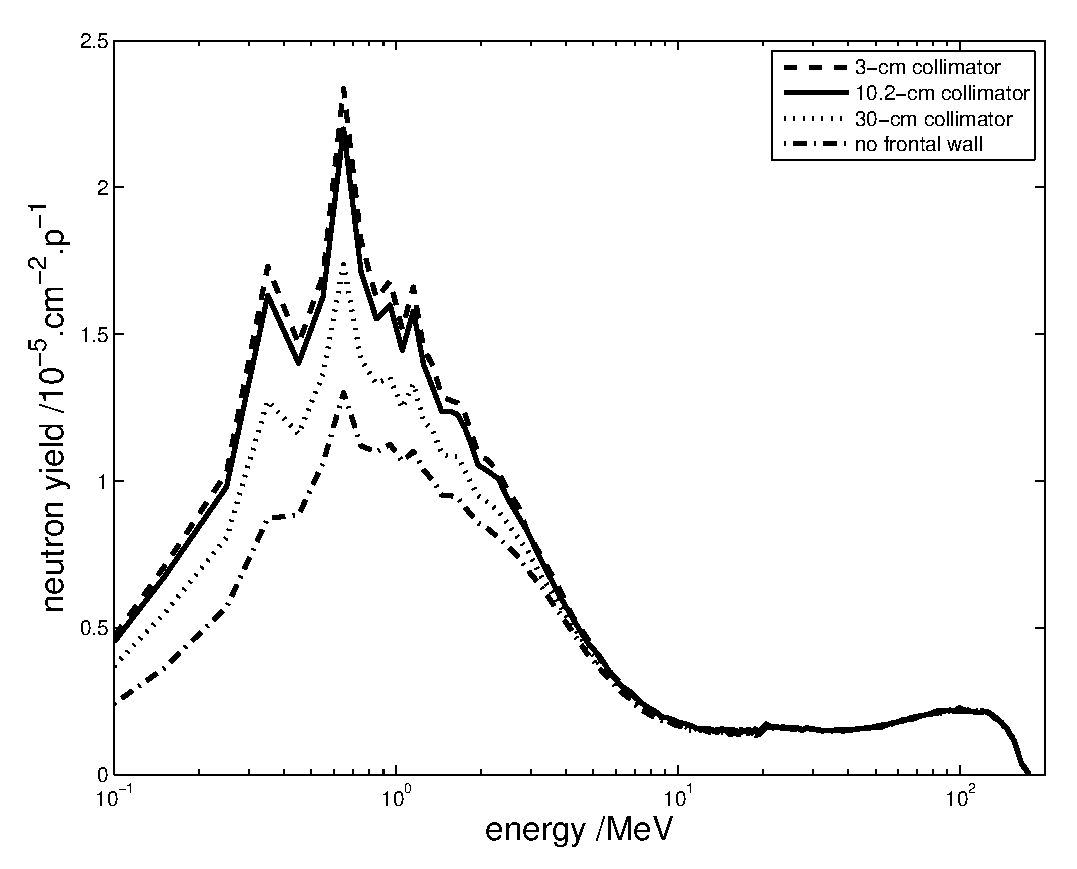
\includegraphics[width=3in]{TOFLethargylinearspace.eps}
	\label{fig:TOFLethargylinearspace}}
	\hfil
	\subfloat[TSL MCNPX modelling~\cite{Prokofiev14}]{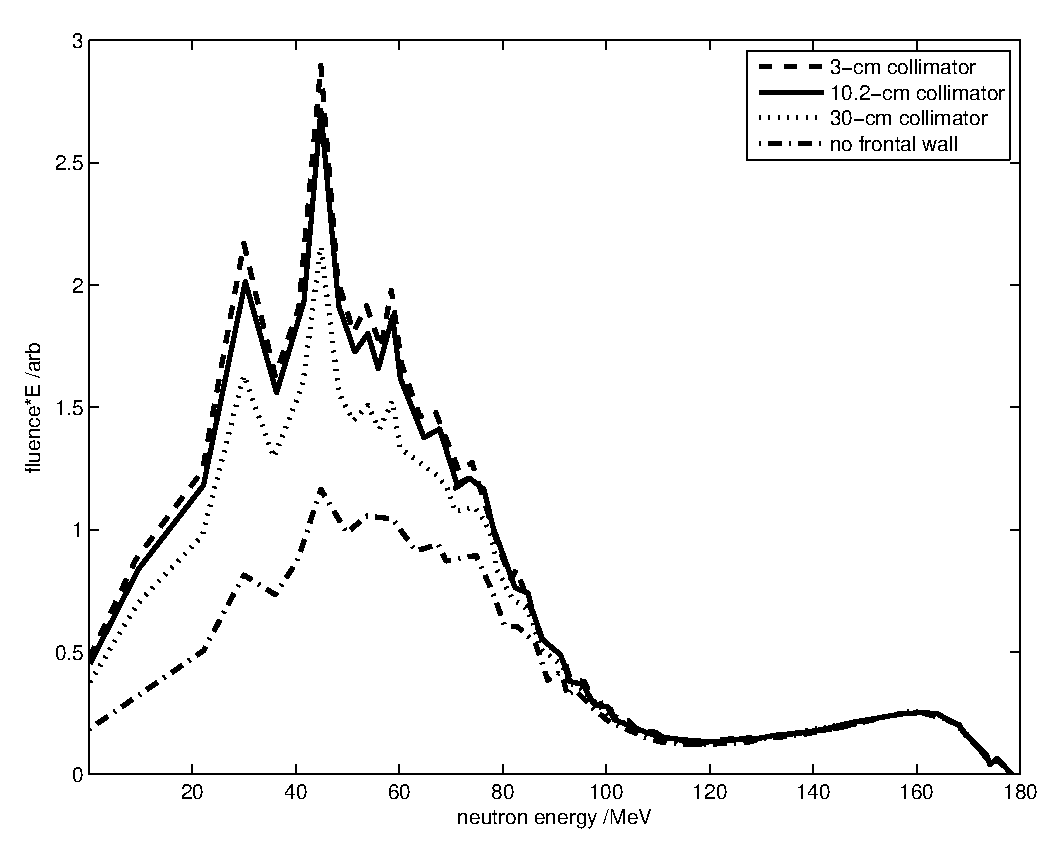
\includegraphics[width=3in]{StandardLetNYieldAtCUPTOF.eps}
	\label{fig:StandardLethargylinearspace}}
	\caption{Simulated spectral fluence at the CUP-TOF position for \SI{3}{\cm}, \SI{10.2}{\cm}, \SI{30}{\cm} and no collimator. The dashed line, solid line, and dotted line represent the neutron yield of collimator with diameter 3, 10.2, and \SI{30}{\cm}. The dash-dotted line represents modelling with no collimator attached.}
	\label{fig_LethargylinearspaceFor4collimators}
\end{figure*}

Fig.~\ref{fig_LethargylinearspaceFor4collimators} shows

\begin{figure}[!t]
	\centering
	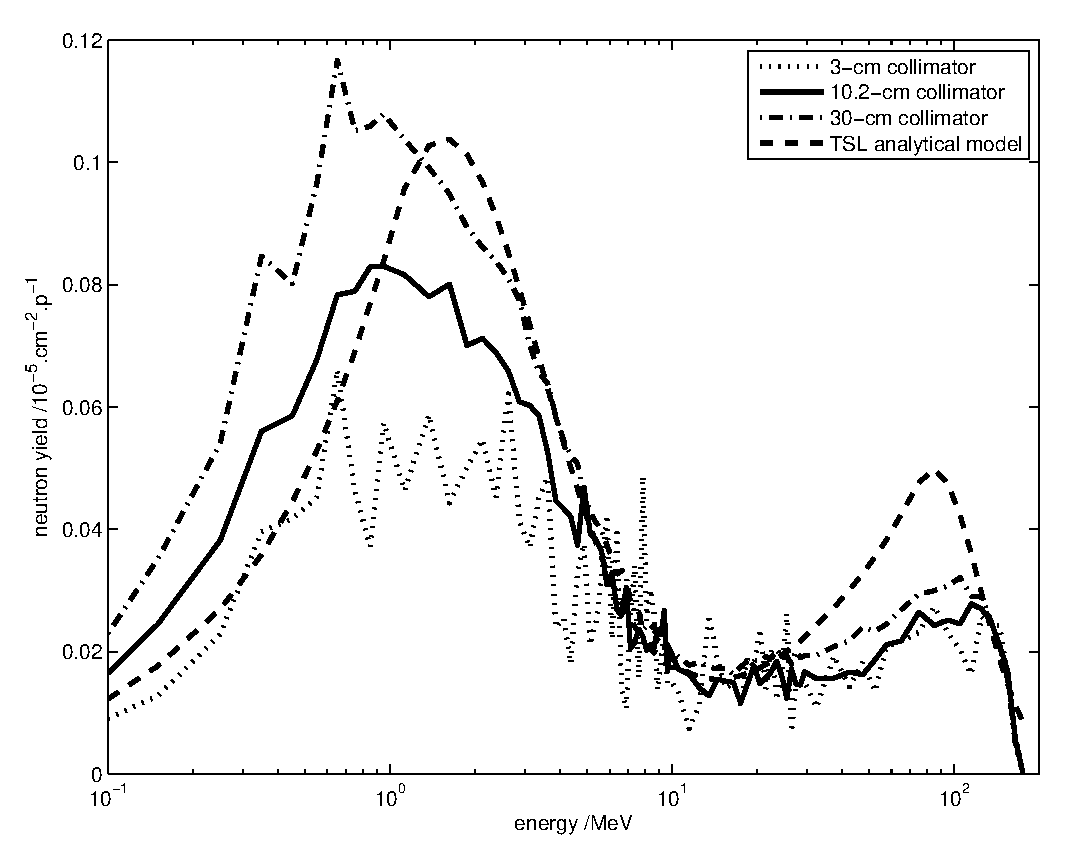
\includegraphics[width=3in]{SUPcomparedlinearspace.eps}
	\caption{Simulated spectral yield at the SUP for \SI{3}{\cm}, \SI{10.2}{\cm}, and \SI{30}{\cm} collimators}
	\label{fig:SUPcomparedlinearspace}
\end{figure}

\subsection{Subsection Two}
\begin{figure*}[!t]
	\centering
	\subfloat[Differential]{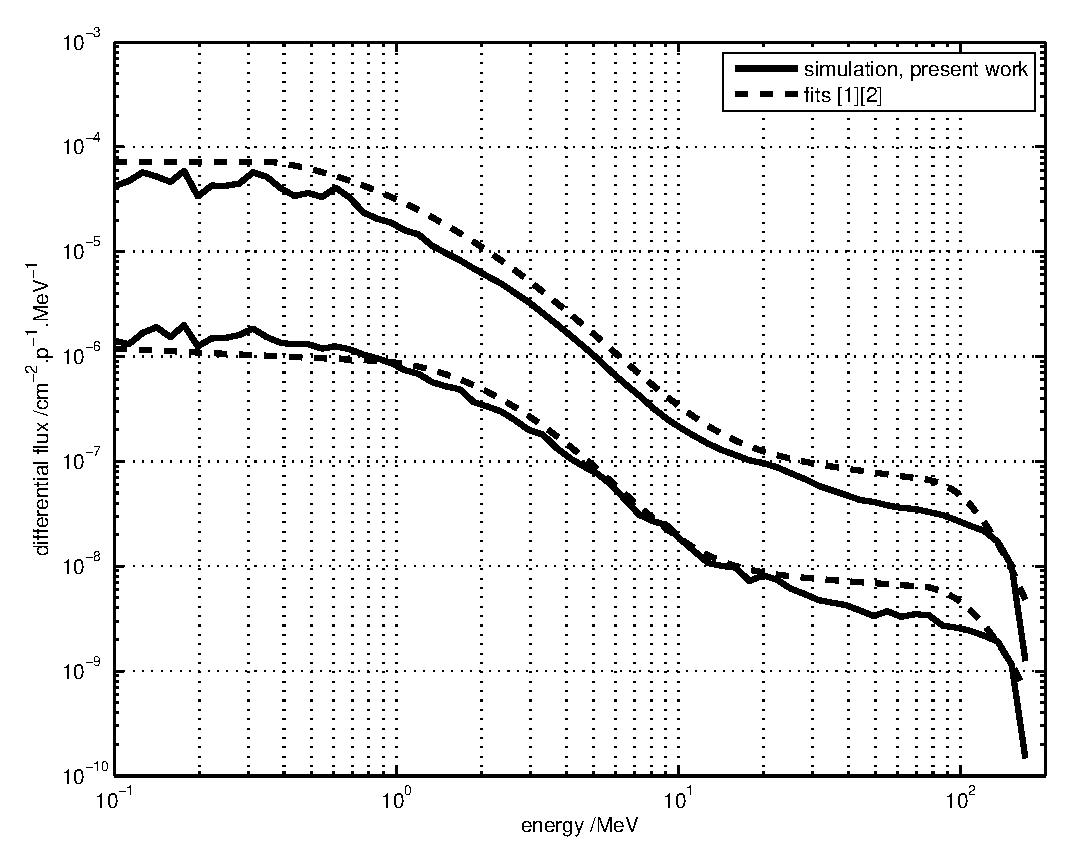
\includegraphics[width=3in]{DiffYieldComparedSUPCUP10.eps}
	\label{fig:DiffYieldComparedSUPCUP10}}
	\hfil
	\subfloat[Integral]{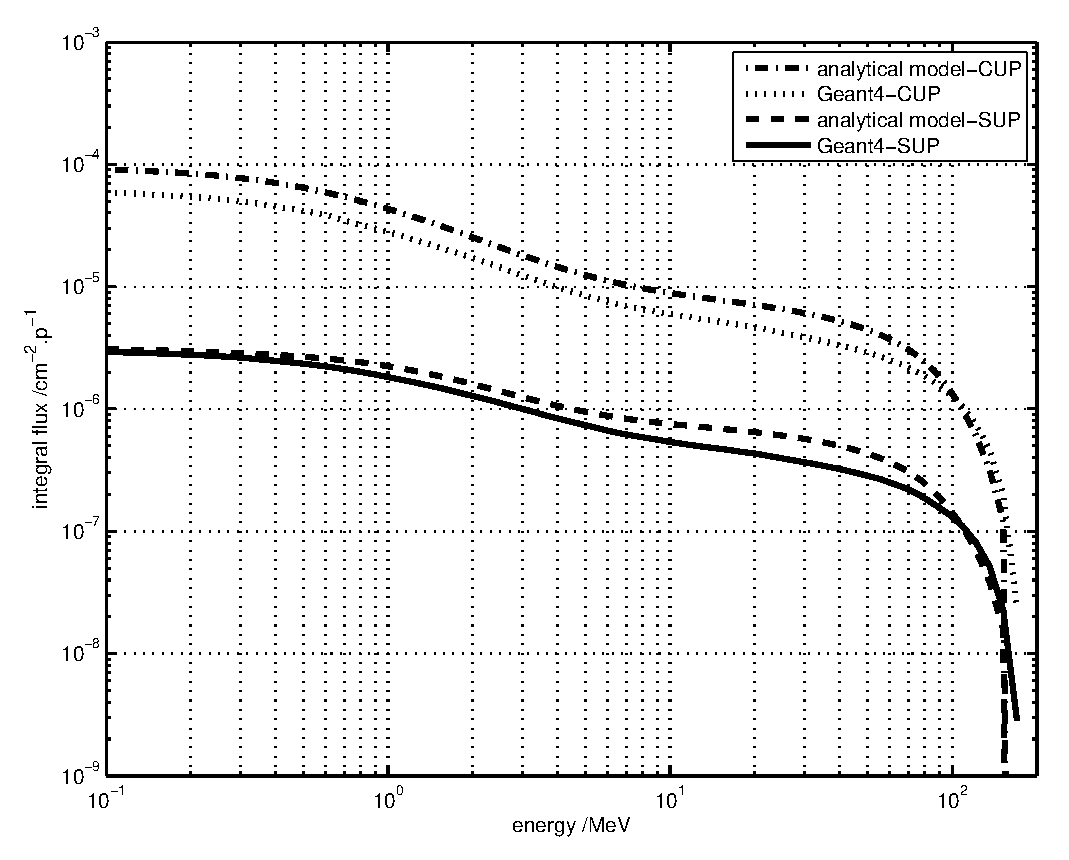
\includegraphics[width=3in]{IntYieldComparedSUPCUP10.eps}
	\label{fig:IntYieldComparedSUPCUP10}}
	\caption{Comparison of Geant4 simulated spectral fluence with analytical model at the SUP and the CUP with \SI{10.2}{\cm} collimator~\cite{Prokofiev2009,Prokofiev14}}
	\label{fig:NYieldComparedSUPCUP10}
\end{figure*}

\subsection{Subsection Three}
\begin{figure}[!t]
	\centering
	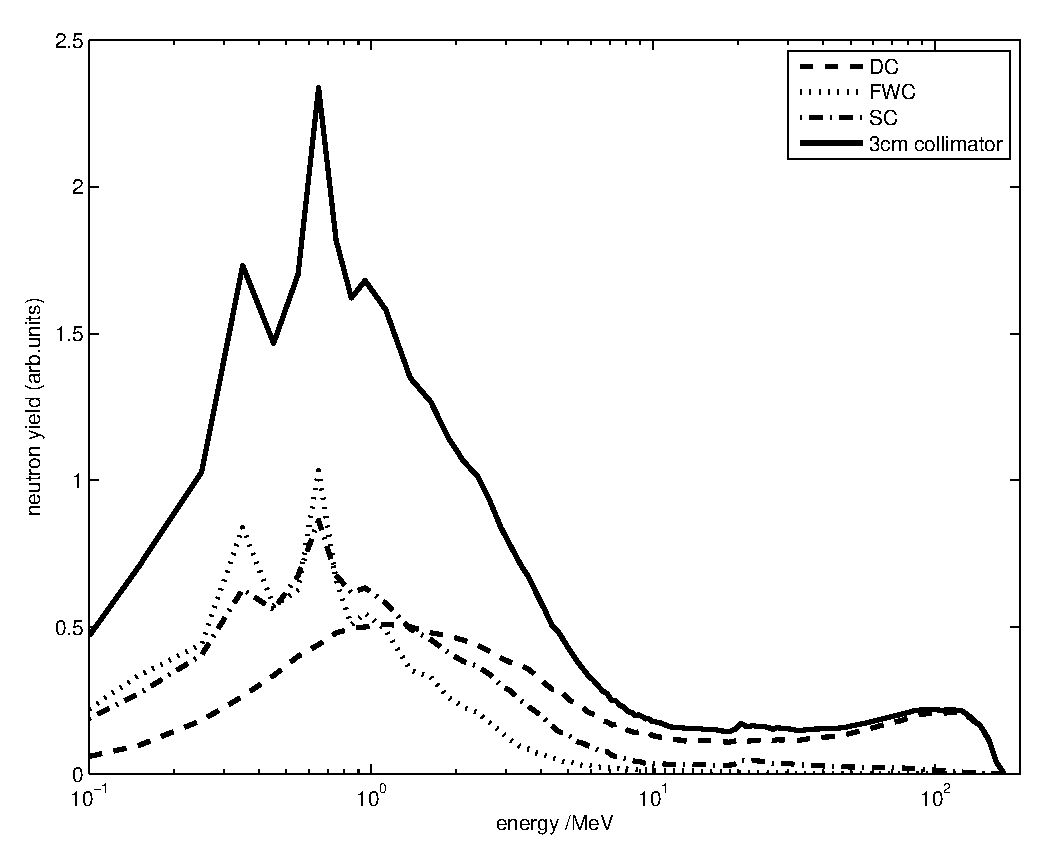
\includegraphics[width=3in]{TOF3Componentslinear.eps}
	\caption{Simulated neutron yield with \SI{3}{\cm} collimator at the CUP-TOF position and three components. The dashed line, dotted line, dash-dotted line represent neutrons directly from the target, frontal wall component, and surroundings component, respectively. The solid line represents the sum of the DC, FWC, and SC components, which is the neutron yield with \SI{3}{\cm} collimator at the CUP-TOF position, in the lethargy scale.}
	\label{fig:TOF3Componentslinear}
\end{figure}

\subsection{Subsection Four, time of flight spectrum}

\begin{figure}[!t]
	\centering
	\subfloat[Time of flight spectrum at the CUP-TOF position, with \SI{3}{\cm} collimator]{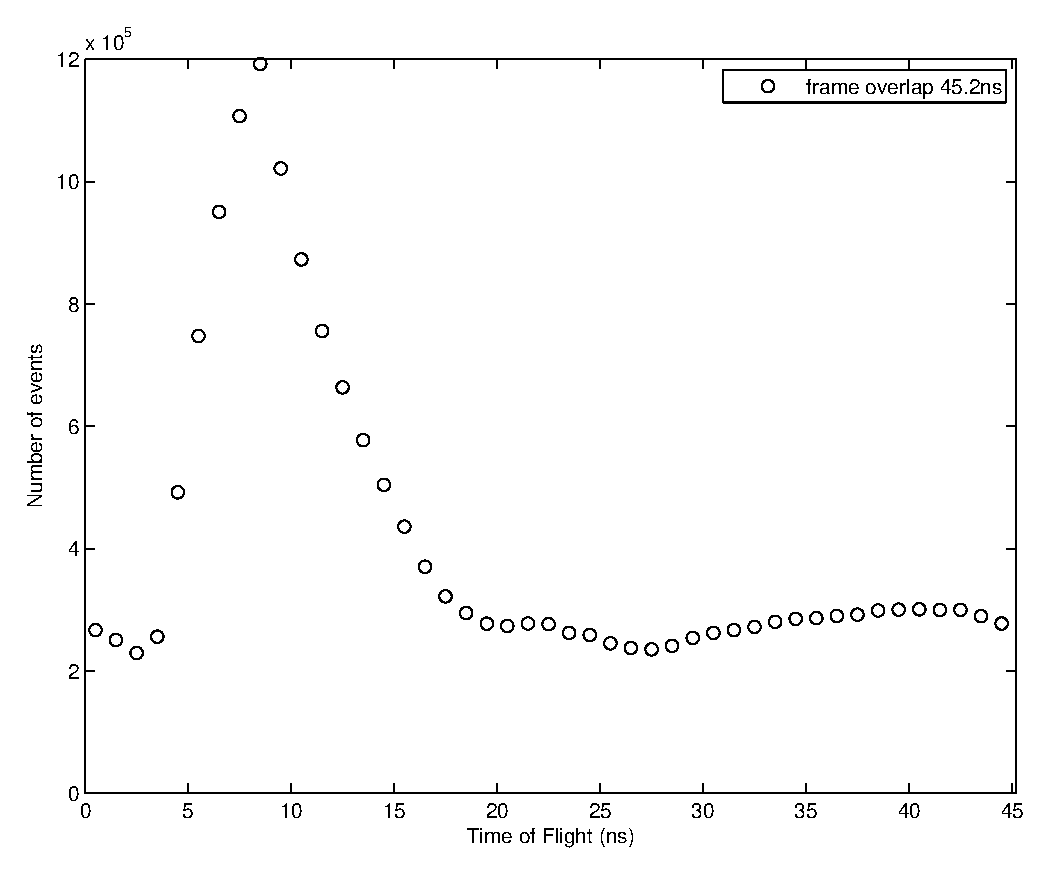
\includegraphics[width=3in]{TOF3frameoverlap.eps}
	\label{fig:TOFFrameOverlapspectrum}}
	\vfil
	\subfloat[Time of flight spectrum at the SUP, with \SI{10.2}{\cm} collimator]{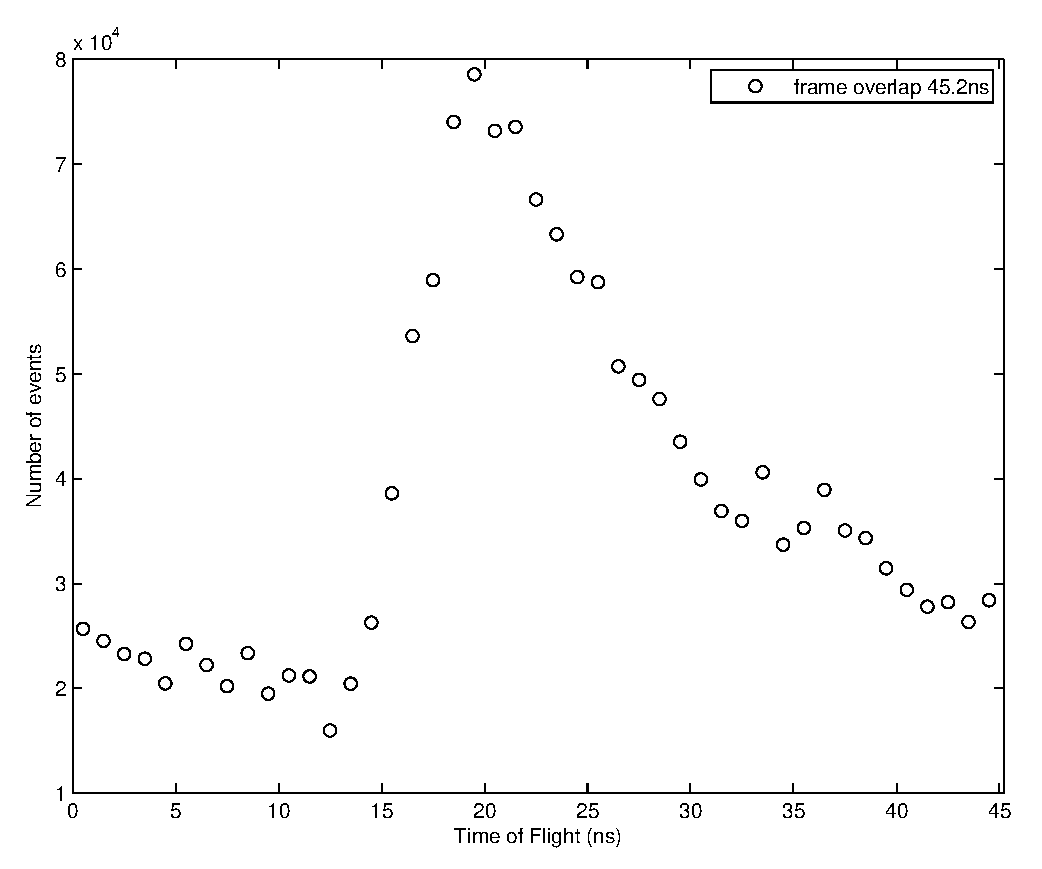
\includegraphics[width=3in]{SUP10frameoverlap.eps}
	\label{fig:SUP10FrameOverlapspectrum}}
\end{figure}

\subsection{Subsection Five, beam profile folding with $^{238}U(n,f)$ cross-section}

\begin{figure}[!t]
	\centering
	\subfloat[\SI{3}{\cm} collimator]{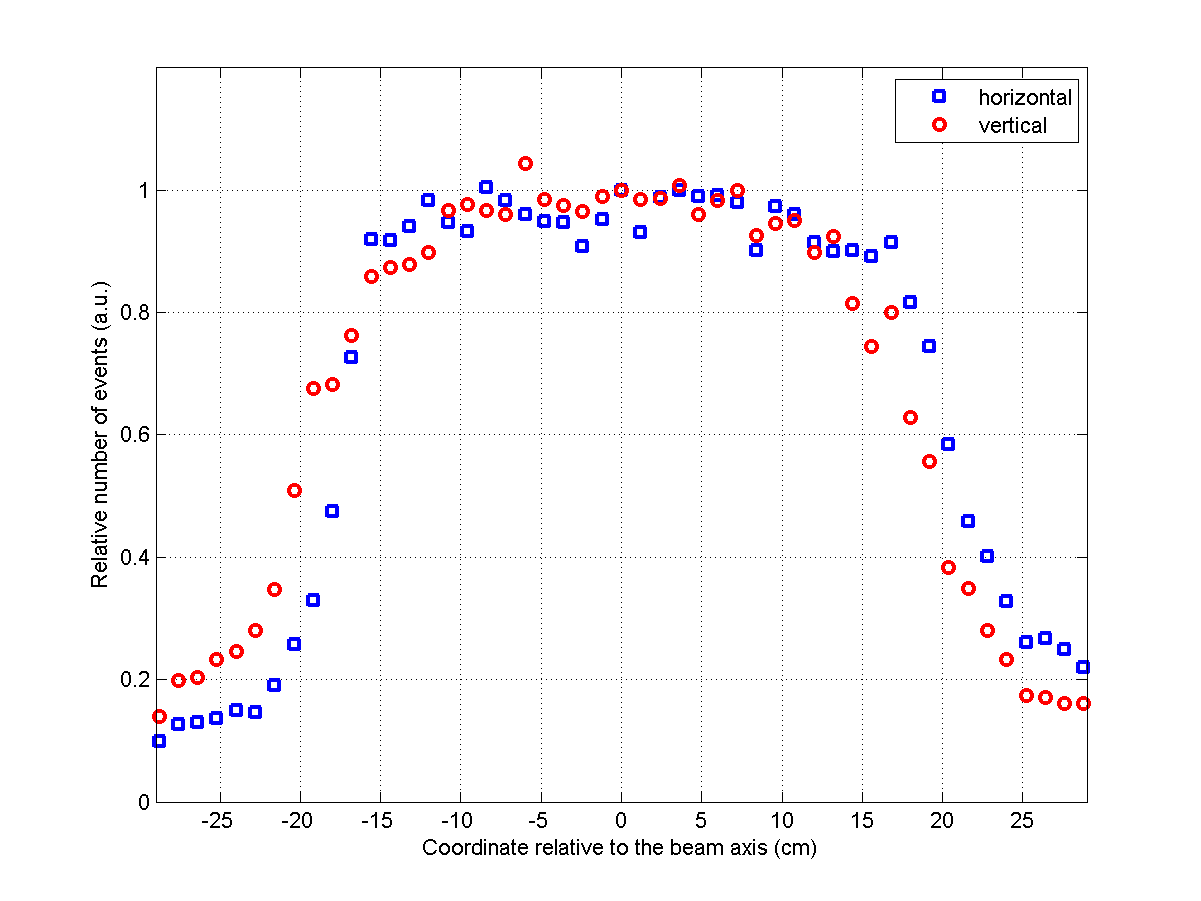
\includegraphics[width=2.5in]{CUPTOF3beampro.png}
	\label{fig:CUPTOF3beampro}}
	\hfil
	\subfloat[\SI{10.2}{\cm} collimator]{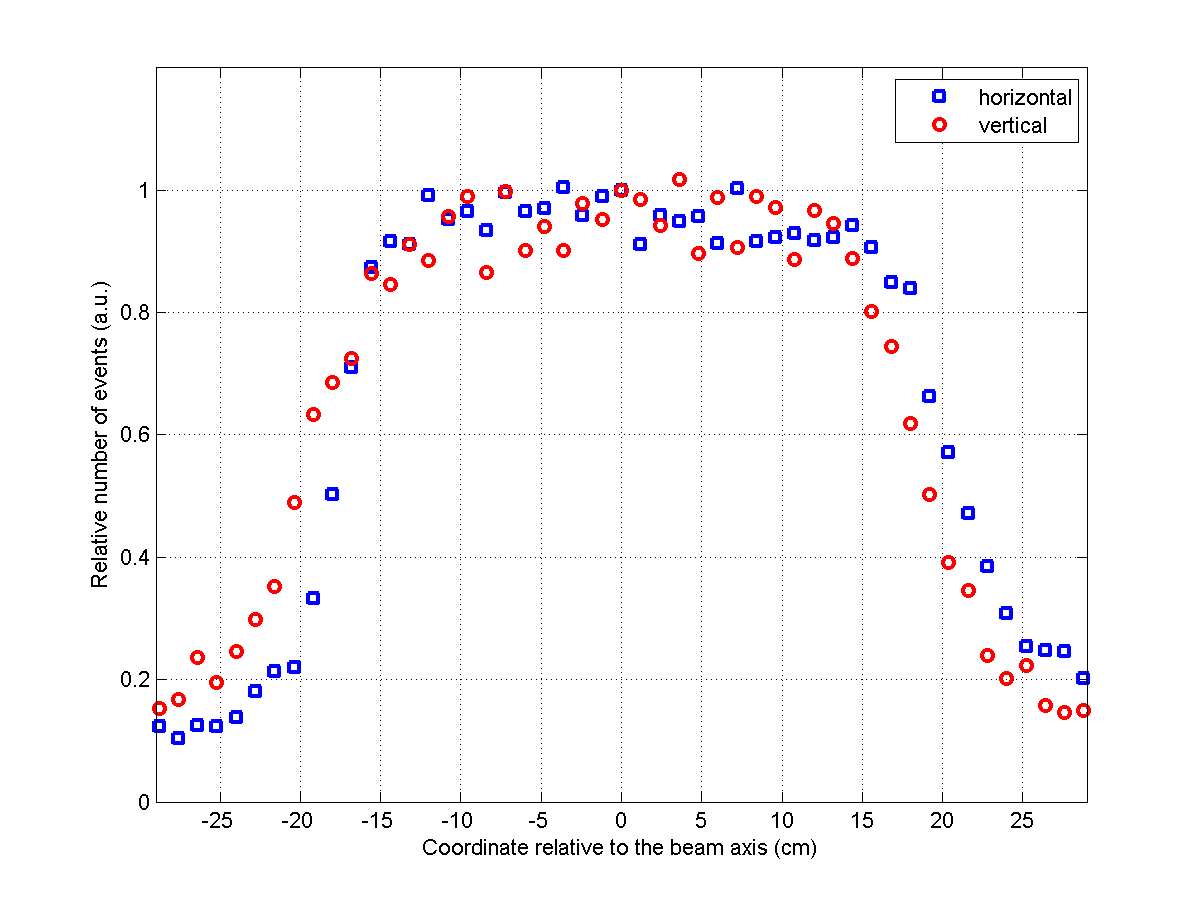
\includegraphics[width=2.5in]{CUPTOF10beampro.png}
	\label{fig:CUPTOF10beampro}}
	\hfil
	\subfloat[\SI{30}{\cm} collimator]{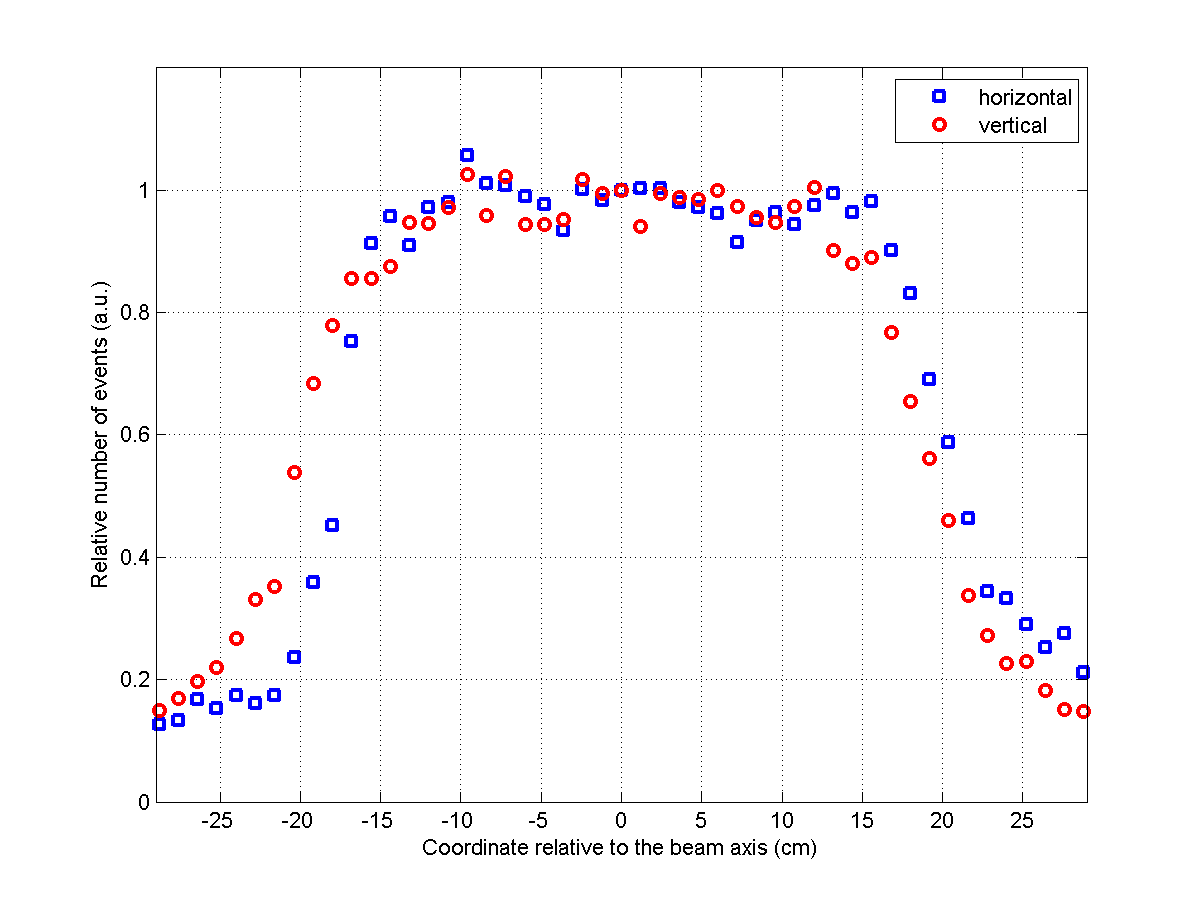
\includegraphics[width=2.5in]{CUPTOF30beampro.png}
	\label{fig:CUPTOF30beampro}}
	\caption{Neutron beam profiles folding with $^{238}U(n,f)$ cross-section at the CUP-TOF position with \SI{3}{\cm}, \SI{10.2}{\cm}, and \SI{30}{\cm} collimator}
	\label{fig:CUPTOFbeamprofileFolding}
\end{figure}

\begin{figure}[!t]
	\centering
	\subfloat[\SI{3}{\cm} collimator]{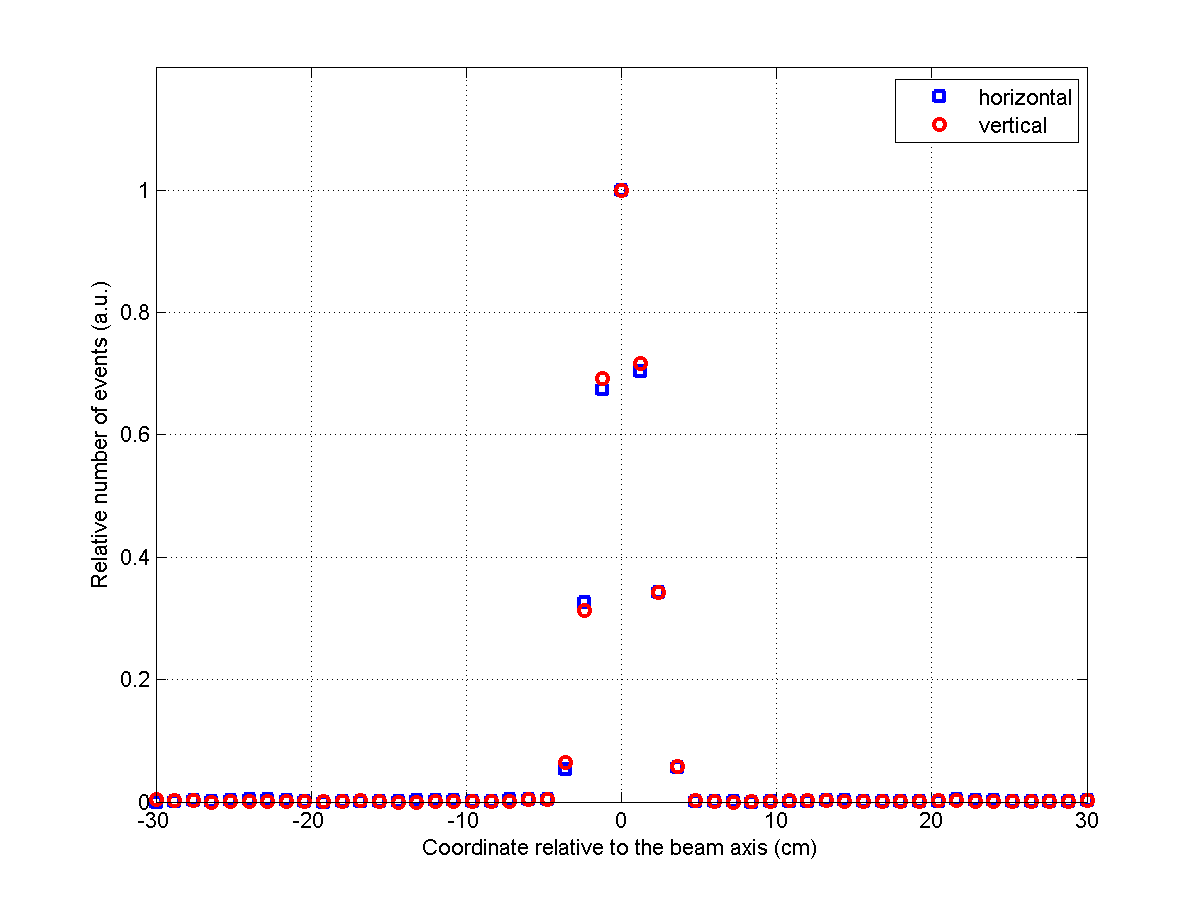
\includegraphics[width=2.5in]{SUP3beamproFolding.png}
	\label{fig:SUP3beamproFolding}}
	\hfill
	\subfloat[\SI{10.2}{\cm} collimator]{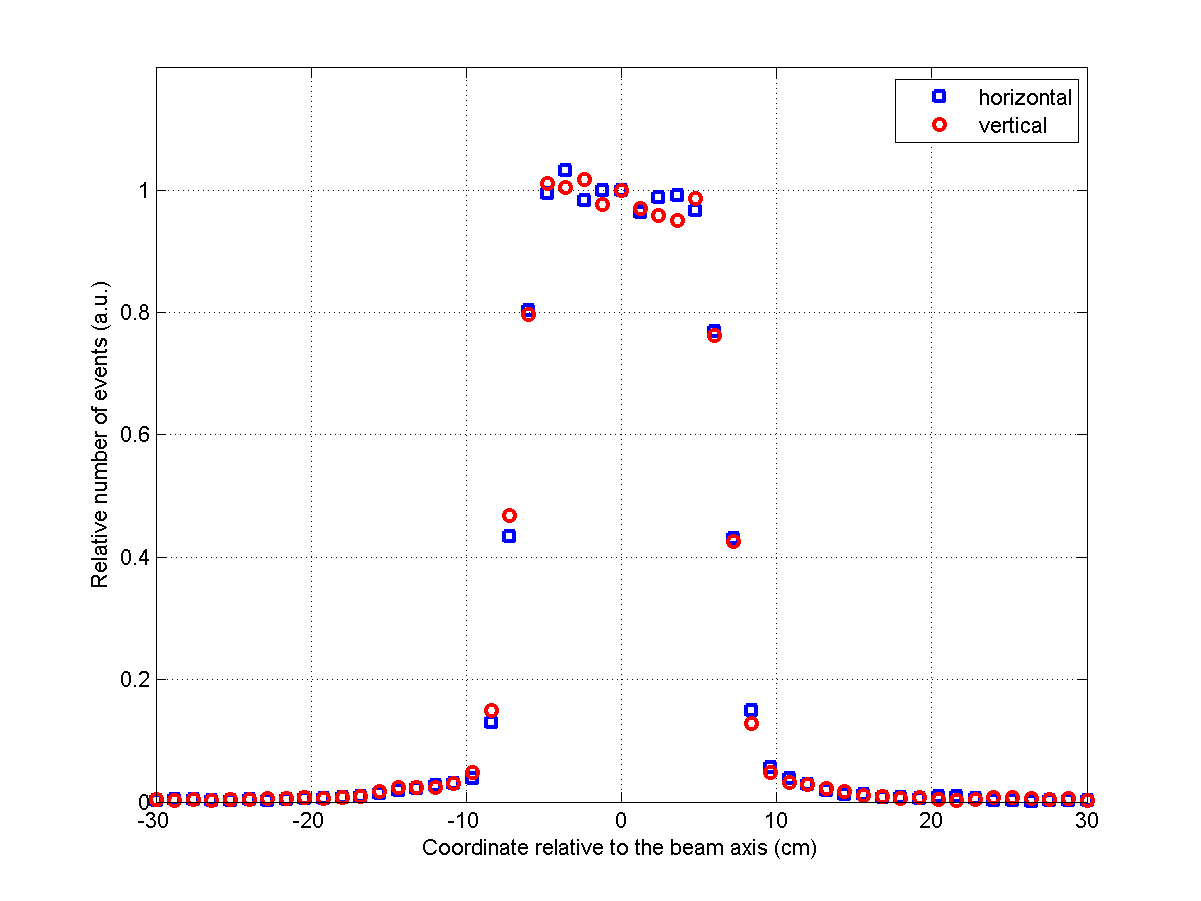
\includegraphics[width=2.5in]{SUP10beamproFolding.png}
	\label{fig:SUP10beamproFolding}}
	\hfill
	\subfloat[\SI{30}{\cm} collimator]{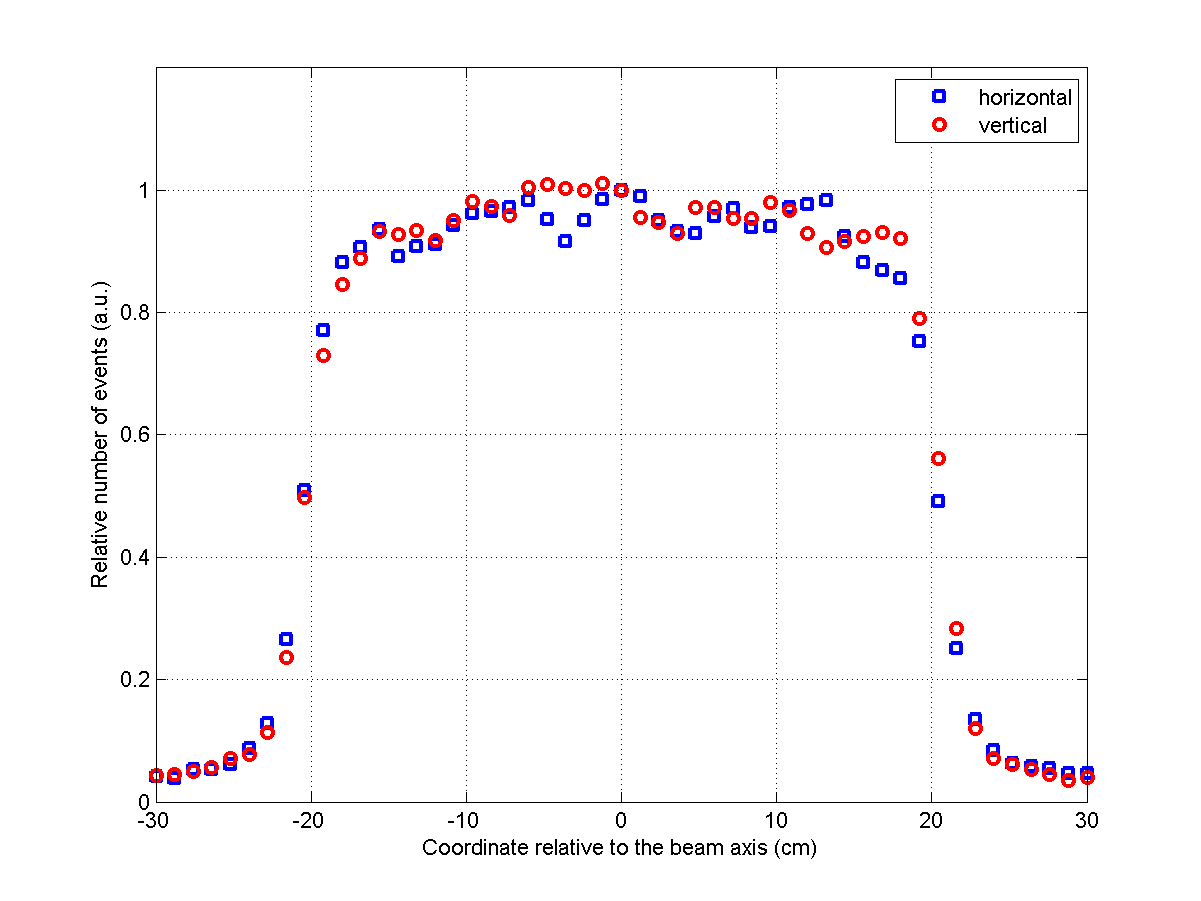
\includegraphics[width=2.5in]{SUP30beamproFolding.png}
	\label{fig:SUP30beamproFolding}}
	\caption{Neutron beam profile folding with $^{238}U(n,f)$ cross-section at the SUP with \SI{3}{\cm}, \SI{10.2}{\cm}, and \SI{30}{\cm} collimator}
	\label{fig:SUPbeamprofileFolding}
\end{figure}

Fig.~\ref{fig:CUPTOFbeamprofileFolding} shows

%\begin{equation}
%\label{eq:emc}
%e = mc^2
%\end{equation}

\subsection{Gamma, subsection one : Spatial distribution}

\begin{figure}[!t]
	\centering
	\subfloat[\SI{3}{\cm} collimator]{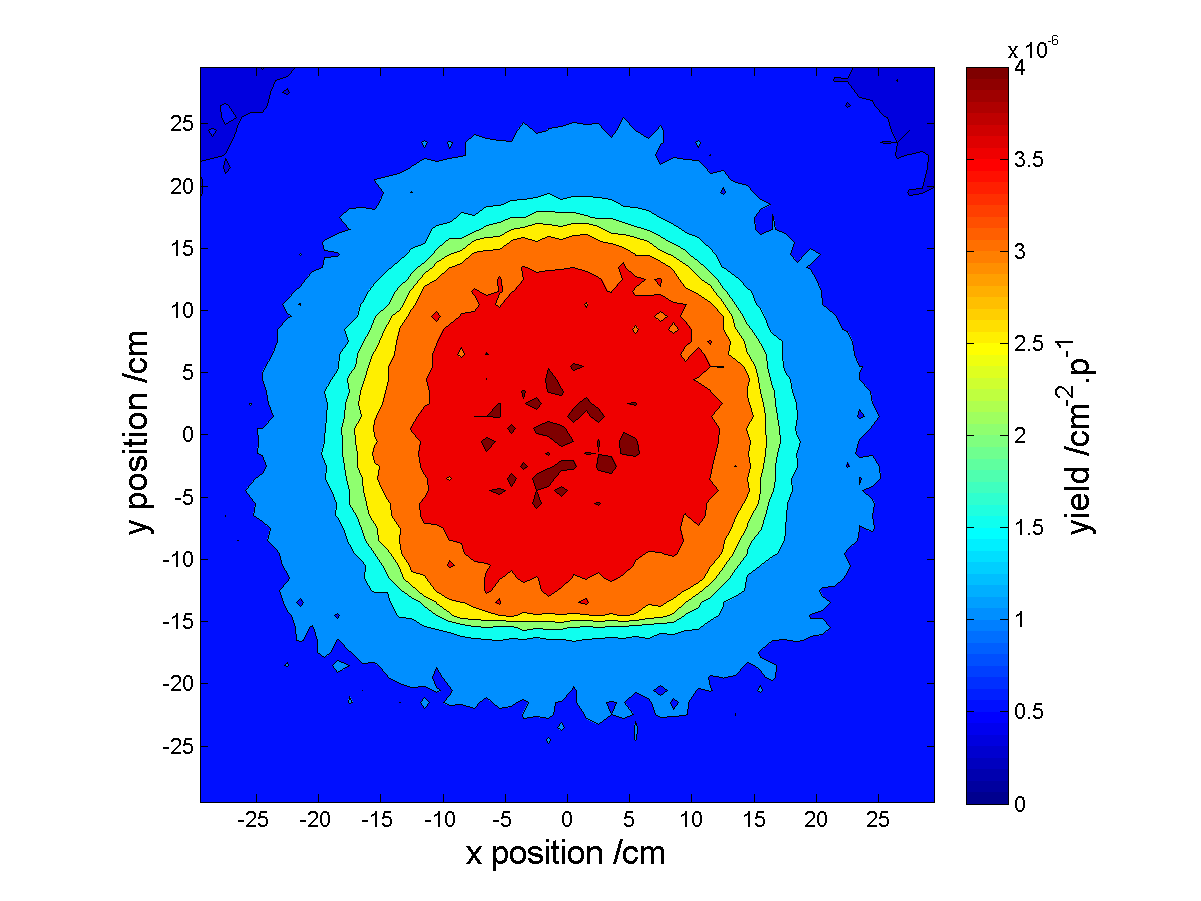
\includegraphics[width=3in]{CUP3ColSpatialDistributionAllG}
	\label{fig:CUP3SpatialDistributionAllG}}
	\hfil
	\subfloat[\SI{10.2}{\cm} collimator]{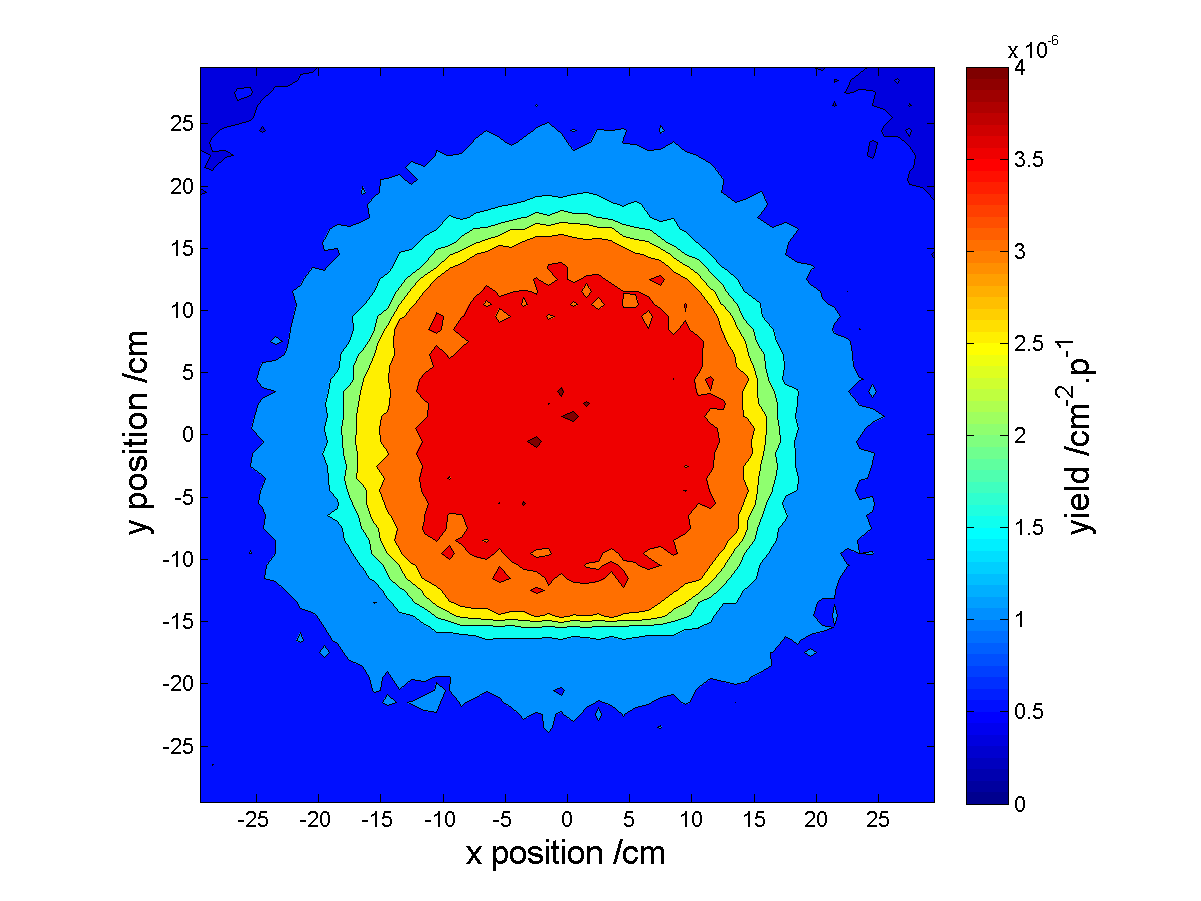
\includegraphics[width=3in]{CUP10ColSpatialDistributionAllG}
	\label{fig:CUP10SpatialDistributionAllG}}
	\caption{Gamma spatial distribution at the CUP with \SI{3}{\cm}, and \SI{10.2}{\cm} collimator~\cite{Prokofiev2009,Prokofiev14}}
	\label{fig:gCUPSpatialDistribution}
\end{figure}


\begin{table}[!tbp]
\caption[{$\gamma$ yield for each collimator in a radius of \SI{5}{\cm} at the CUP}]{$\gamma$ yield for each collimator at the CUP}	%title of the table
\centering
\label{table:GYieldCUP}
\begin{tabular}{lcc}
	\hline% insert double-line
	Collimator size   & above \SI{1}{\MeV}   &  above \SI{0.1}{\MeV}  \\
	\cmidrule(r){2-3}
/\si{\cm}       & /\SI{e-6}{\photon\per\cm\squared\per\proton} & /\SI{e-6}{\photon\per\cm\squared\per\proton} \\
\hline % insert single-line
3 & 4.93 & 15.73\\

10.2 & 4.86  &  15.27\\

30 & 4.44  &  13.80\\
\hline
\end{tabular}
\end{table}

\begin{table}[!tbp]
\caption[$\gamma$ yield for each collimator in umbra region at the SUP]{$\gamma$ yield for each collimator in umbra region at the SUP}	%title of the table
\centering
\label{table:GYieldSUP}
\begin{tabular}{l	c	c}
\hline% insert double-line
Collimator size   & above \SI{1}{\MeV}   &  above \SI{0.1}{\MeV}   \\
\cmidrule(r){2-3}
/\si{\cm}       & \/\SI{e-6}{\photon\per\cm\squared\per\proton} &  /\SI{e-6}{\photon\per\cm\squared\per\proton} \\
\hline % insert single-line
3 & 2.3 & 6.7\\

10.2 & 2.8  &  8.3\\

30 & 3.2  &  9.4\\
\hline
\end{tabular}
\end{table}


\subsection{Gamma, subsection two : Photon spectra at the CUP and SUP }

\begin{figure}[!t]
	\centering
	\subfloat[CUP]{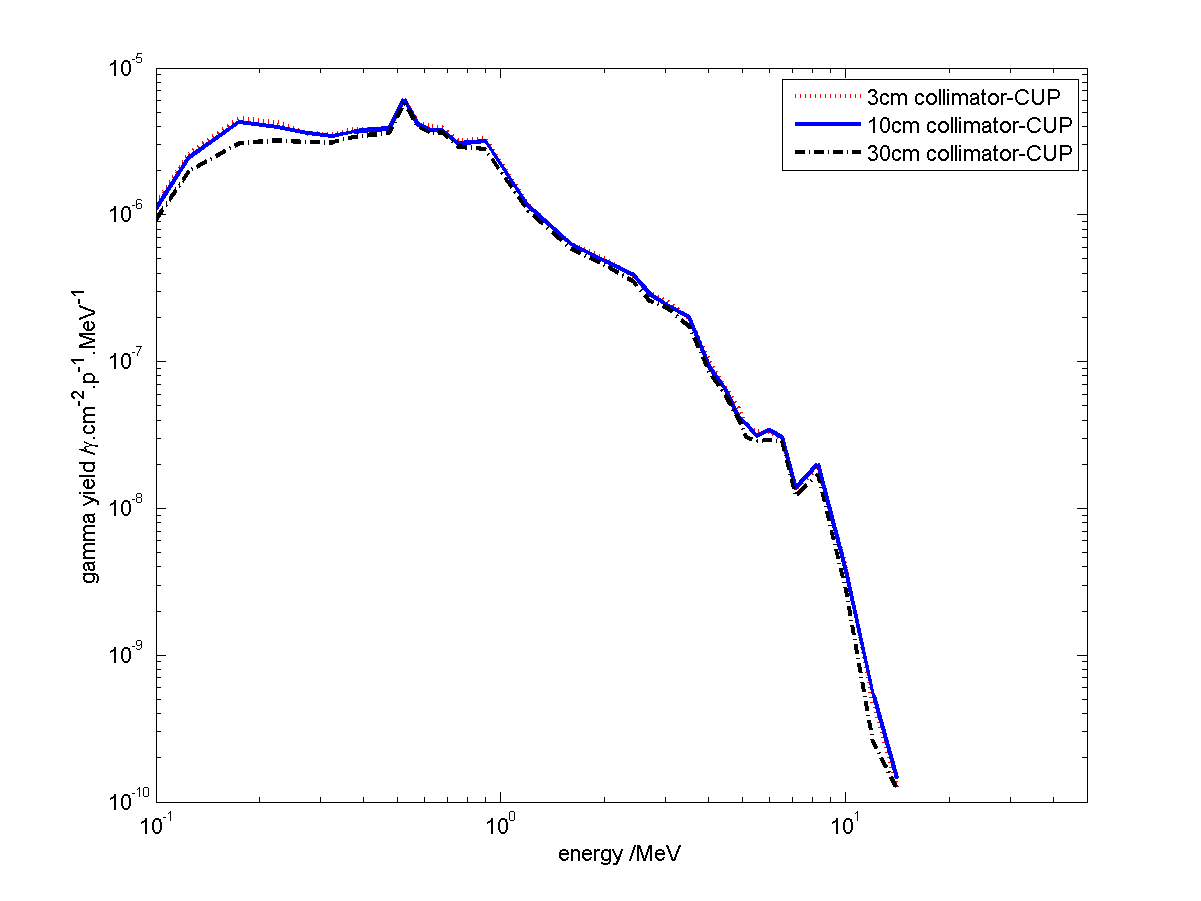
\includegraphics[width=3in]{gCUPDYieldcompared}
	\label{fig:gCUPDYieldcompared}}
	\vfil
	\subfloat[SUP]{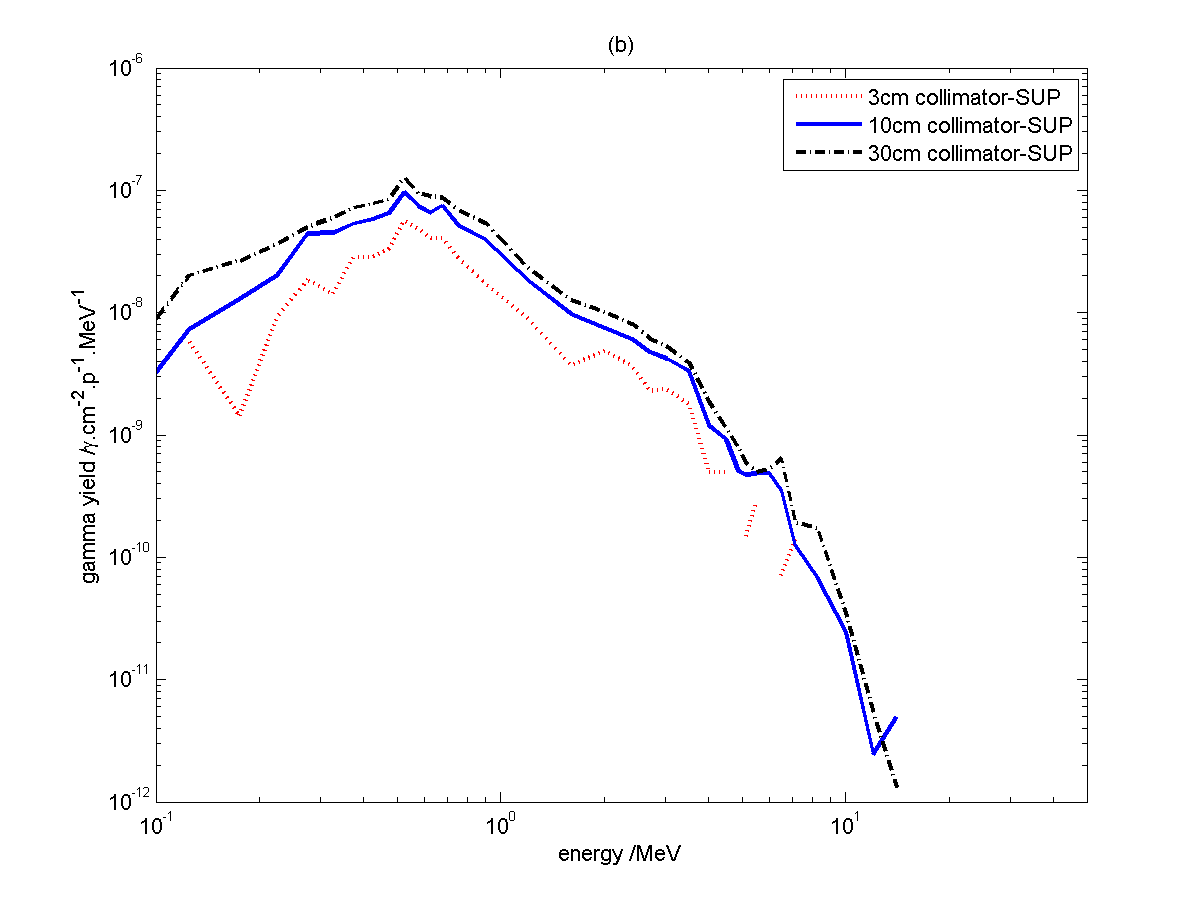
\includegraphics[width=3in]{gSUPDYieldcompared}
	\label{fig:gSUPDYieldcompared}}
	\caption{Comparison of differential photon yield at the CUP and SUP}
	\label{fig:gDYieldspectra}
\end{figure}

\begin{figure}[!t]
	\centering
	\subfloat[CUP]{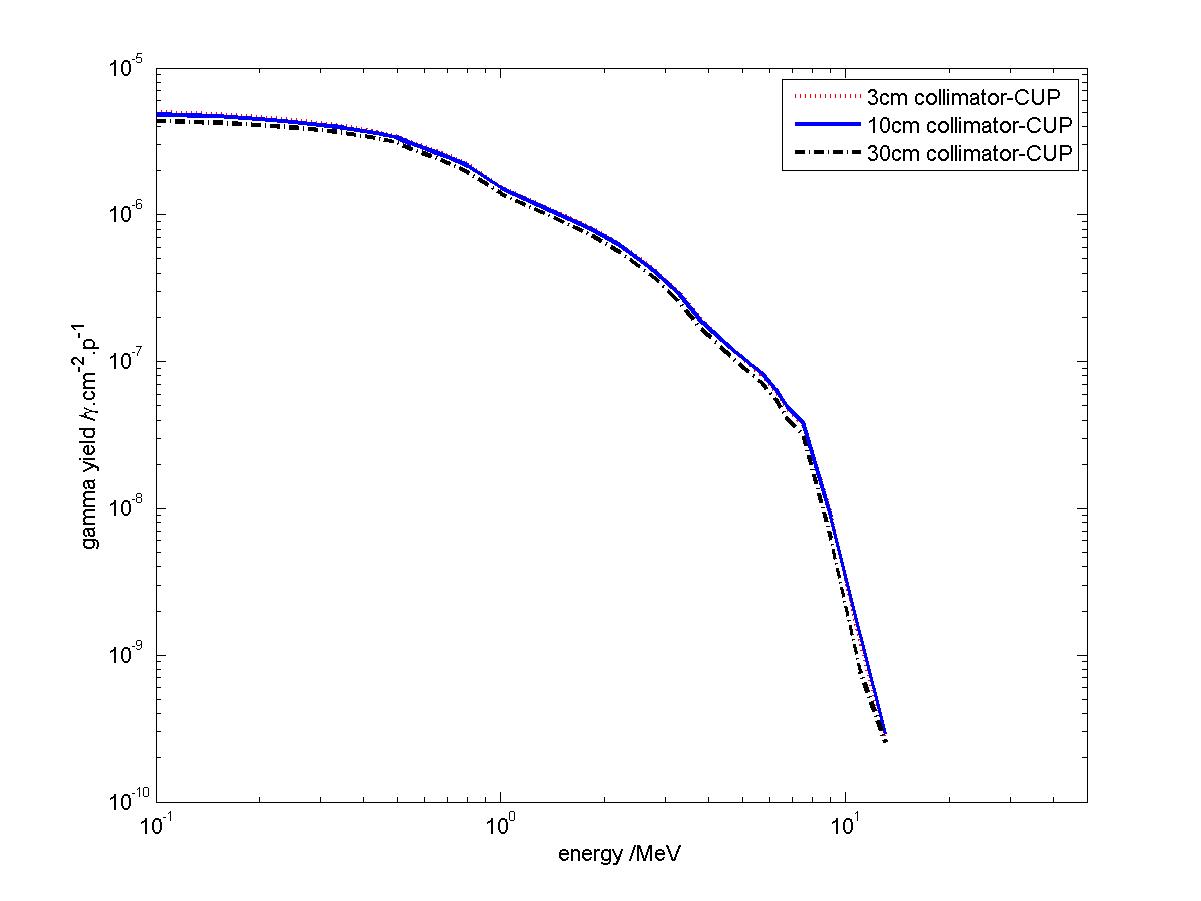
\includegraphics[width=3in]{gCUPIYieldcompared}
	\label{fig:gCUPIYieldcompared}}
	\vfil
	\subfloat[SUP]{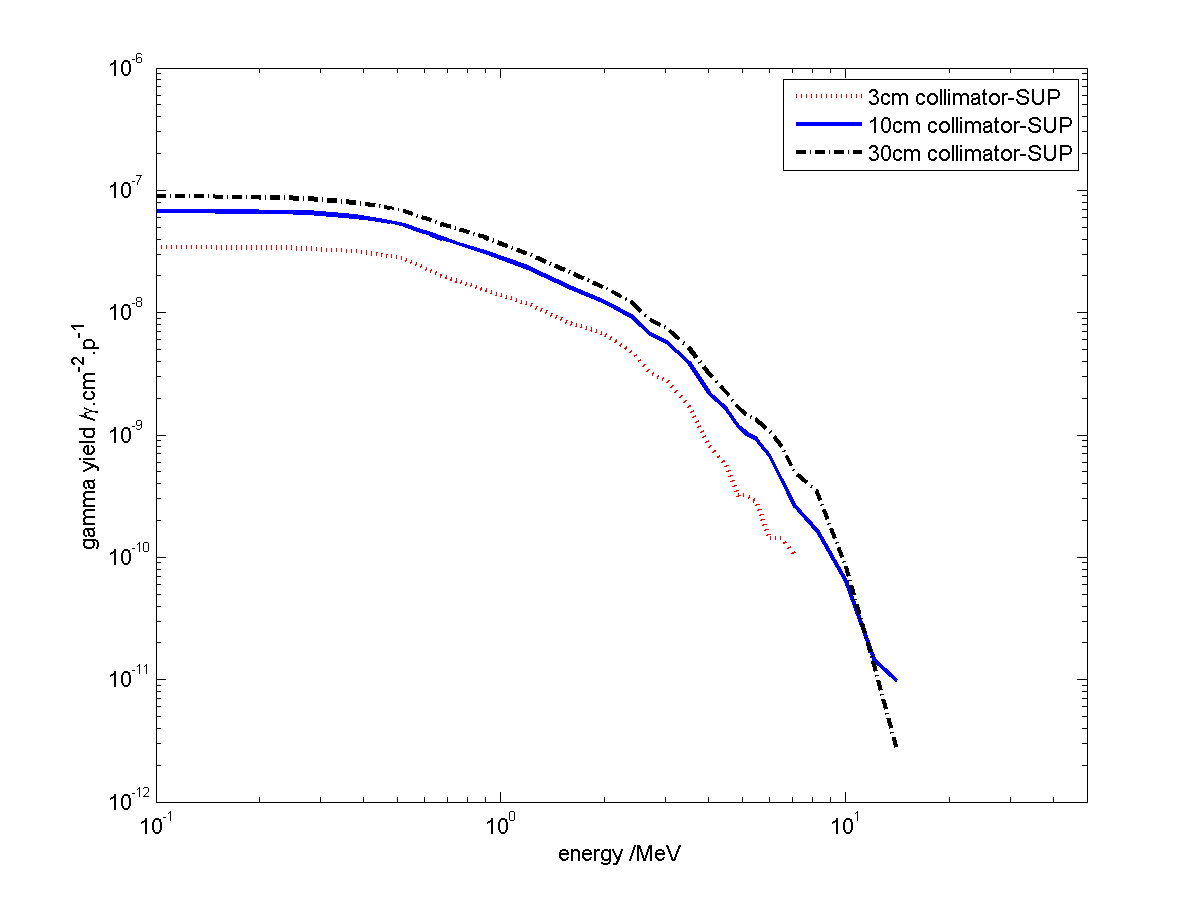
\includegraphics[width=3in]{gSUPIYieldcompared}
	\label{fig:gSUPIYieldcompared}}
	\caption{Comparison of integral photon yield at the CUP and SUP}
	\label{fig:gIYieldspectra}
\end{figure}
Figure~\ref{fig:gIYieldspectra} displayed integral photon spectra at the CUP and SUP. The photon spectra at the SUP with \SI{3}{\cm} collimator, it is dominated by energy within about \SI{7}{\MeV} at the SUP, see Figure~\ref{fig:gSUPIYieldcompared}.

\begin{table}
\caption{$\gamma$ dose rate for each collimator at the CUP and SUP}	%title of the table
\centering
\label{Table:DoseRate}
        \begin{tabular}{l c c}
            \toprule
            {collimator diameter}   &{CUP}         &{SUP}\\
            {\si{\centi\metre}}    &{\si{mSvh^{-1}}}   &{\si{mSvh^{-1}}}\\
            \midrule
            3                       & 378.0                	& 17.32\\
            10.2                  & 369.4               	& 20.90\\
            30                     & 336.4          		& 23.65\\
            \bottomrule
\end{tabular}
\end{table}


\begin{figure}[!t]
	\centering
	\subfloat[CUP]{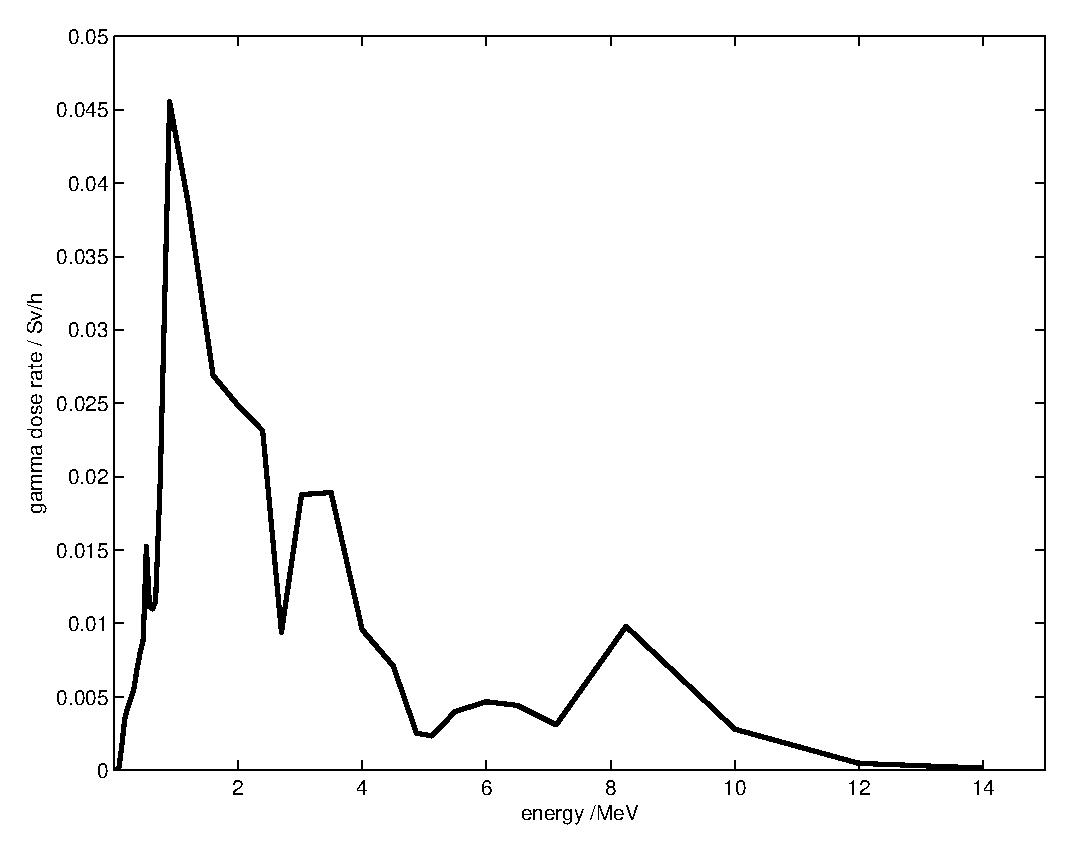
\includegraphics[width=2.5in]{DoseVSenergyCUP.eps}
	\label{fig:DoseVSenergyCUP}}
	\hfil
	\subfloat[SUP]{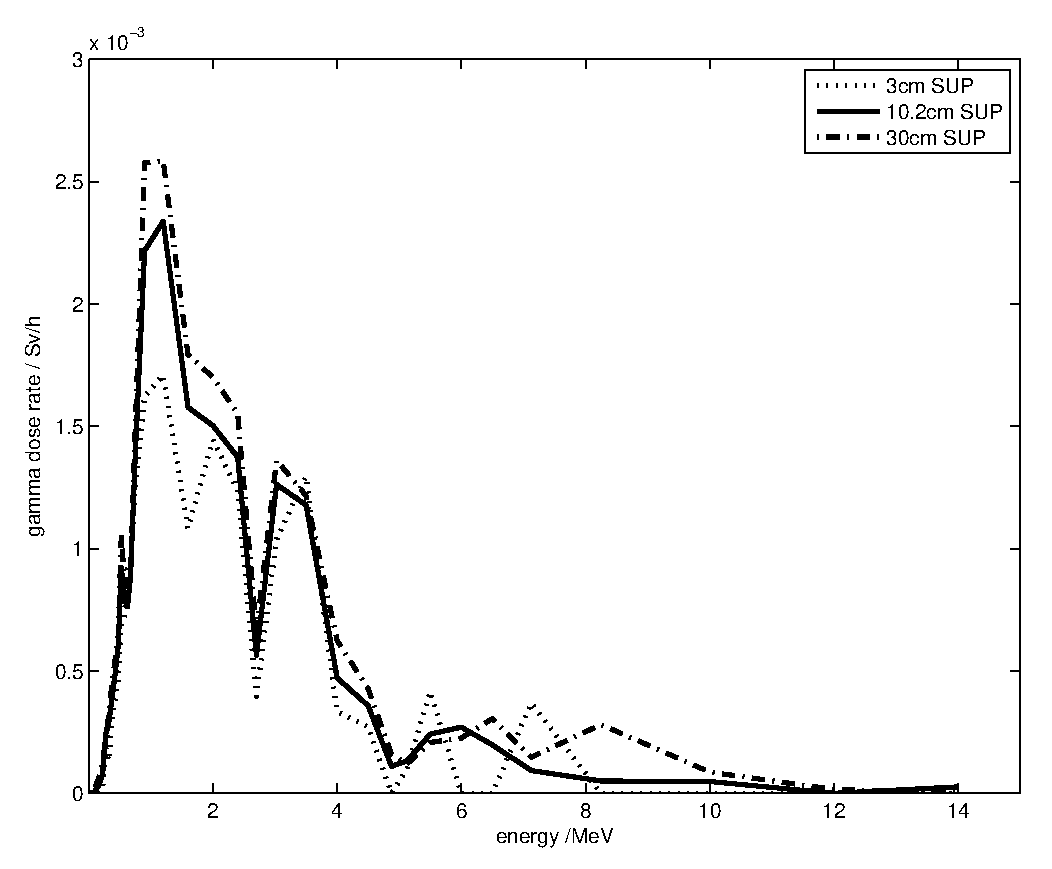
\includegraphics[width=2.5in]{DoseVSenergySUP.eps}
	\label{fig:DoseVSenergySUP}}
	\caption{Dose versus energy at the CUP and SUP with \SI{3}{\cm}, \SI{10.2}{\cm}, and \SI{30}{\cm} collimators}
	\label{fig:DoseVSenergy}
\end{figure}

%------------------------------------------------
\section{Discussion}

\subsection{Subsection One}

Neutron .....

\subsection{Subsection Two}

Gamma .....

%----------------------------------------------------------------------------------------
%	REFERENCE LIST
%----------------------------------------------------------------------------------------

\ifCLASSOPTIONcaptionsoff
  \newpage
\fi

\begin{thebibliography}{99} % Bibliography - this is intentionally simple in this template

\bibitem{Wender87}
S.A. Wender and P.W. Lisowski,
\newblock A white neutron source from 1 to 400 MeV,								% title	
\newblock {\em Nucl. Instr. Meth. Phys. Res. B}, vol. 24-25, pp. 897-900.					% vol:page, 2011

\bibitem{Platt13}
Platt, S.P. and Hong, Q. and Mein, S.J. and Zhang, L.H.,
\newblock Neutron and gamma fields at neutron spallation sources for single-event-effects testing,		% title	
\newblock {\em in Proc. 14th European Conf. Radiat. Effects Compon. Syst. 2013,} pp 1-4			% vol:page, 2011

\bibitem{Prokofiev14}
Prokofiev, A.V. and Blomgren, J. and Majerle, M. and Nolte, R. and Rottger, S. and Platt, S.P. and Cai Xiao Xiao and Smirnov, A.N.,
\newblock Characterization of the ANITA Neutron Source for Accelerated SEE Testing at the Svedberg Laboratory,		% title	
\newblock {\em in Proc. IEEE Radiation Effects Data Workshop. 2009,} pp 166-173 							% vol:page, 2011

\bibitem{Prokofiev2009}
Prokofiev, A.V. and Passoth, E. and Hjalmarsson, A. and Majerle, M.,
\newblock CUP-A New High-Flux Irradiation Position at the ANITA Neutron Facility at TSL,		% title	
\newblock {\em in Proc. IEEE Trans. Nucl. Sci. 2014}, pp 1929-1936 					% vol:page, 2011

\end{thebibliography}

%----------------------------------------------------------------------------------------

\todos

\end{document}